\documentclass[12pt]{article}

\usepackage{main}

\begin{document}
	\maketitle
	This model was proposed by \citeA{stock1988probability}  formalises the idea that  the reference cycle is best measured  by looking at co-movements  across several aggregate time series rather than just a single variable, like GDP or  GNP. Importantly, we are here talking about one single but unobserved variable, ``the state of the economy'', denoted here by $C_t$, which can be proxied, according to \cite{stock1988probability, stock&watson1989indexes}, by the experimental CEI.
	
	An important assumption here is that each roughly coincident series has a component that is attributable to the single unobserved variable and a component which is unique  (idosyncratic component), with all of the idiosyncratic omponents of each observed variable being uncorrelated. Those idiosyncratic components are also assumed to be uncorrelated with $C_t$ at all leads and lags. Our goal here is thus to study an ``unobserved single index" or ```dynamic factor" model.
	
	\section{The Coincident Index: The Model }
		The model for the Coincident Economic Indicators \cite{stock&watson1989indexes} is
\begin{equation}
	\begin{aligned}
		\Delta Y_t& = \beta + \gamma(L) \Delta C_t + u_t \\
		D(L) u_t &= \varepsilon_t\\
		\phi(L) \Delta  C_t& = \delta + \eta_t,
	\end{aligned}
\end{equation}
where $L$ denotes the lag operator, and $\phi(L)$, $\gamma(L)$ and $D(L)$ are respectively scalar, vector, and matrix lag polinomials. Following the spirit of \citeA{stock1988probability}, we take $\gamma(L) = \gamma\in\R^n$, where $n$ is the number of variables used in $Y_t$, and $Y_t$ is the vector of logarithms. For simplicity, and again in the spirit of \citeA{stock1988probability}, we take the degree of $\phi$ to be $p=2$ and the degree of $D(L)$ to be $k=2$. Note that the latter is a matrix of lag polinomials. For simplicity, this matrix is assumed to be diagonal, i.e., $D(L) = \text{diag}\left(d_1(L),\ldots, d_k(L)\right)$. Now, let's write our equations in the state space in order to view it as a Kalman filter.

The transition equation for the state is  given by
\begin{equation}
	\begin{bmatrix}
		C_t^\ast \\ u_t^\ast \\ C_{t-1}
	\end{bmatrix}
	=
	\begin{bmatrix}
		\Phi^\ast & 0 & 0 \\ 0 & D^\ast & 0 \\ Z_c & 0 & 1
	\end{bmatrix}
	\begin{bmatrix}
		C_{t-1}^\ast \\ u_{t-1}^\ast \\ C_{t-1}
	\end{bmatrix}
	+ 
	\begin{bmatrix}
		Z_c & 0 \\ 0 & Z_u \\ 0 & 0
	\end{bmatrix}
	\begin{bmatrix}
		\eta_t \\ \varepsilon_t
	\end{bmatrix}
\end{equation}
where 
\begin{equation}
	\begin{aligned}
		C_{t}^\ast &= 
		\begin{bmatrix}
			\Delta C_t &	\Delta C_{t-1} &\cdots \Delta C_{t-p+1}
		\end{bmatrix}'
		\\
		u_t^\ast &= 
		\begin{bmatrix}
			u_t' & u_{t-1}' & \cdots & u_{t-k+1}'
		\end{bmatrix}'
		\\
		\Phi^\ast &=
		\begin{bmatrix}
			\begin{matrix}
				\phi_1 & \cdots  &\phi_{p-1} &
			\end{matrix} & \phi_p\\
			I_{p-1} & 0 
		\end{bmatrix}
		\\
		D^\ast &=
		\begin{bmatrix}
			\begin{matrix}
				D_1  & \cdots & D_{k-1} 
			\end{matrix}& D_k\\
			I_{n(k-1)} & 0 
		\end{bmatrix}
	\end{aligned}
\end{equation}
and
\begin{equation}
	\begin{aligned}
		Z_c & = \begin{bmatrix}
			1 & 0_{1\times(p-1)}
		\end{bmatrix}\\
		Z_u & = \begin{bmatrix}
			I_n & 0_{n\times n (k-1)}
		\end{bmatrix}
	\end{aligned}
\end{equation}
and where $I_n$ denotes the $n\times n$ identity matrix, $0_{n\times k}$ denotes a $n\times k$ matrix of zeros, and $D_i = \text{diag}(d_{1,i}, \ldots, d_{n,i}$), where $d_j(L) = 1- \sum_{i=1}^k d_{j,i} L^i$. Note that we are augmenting our vector to be able to recover $C_t$ as $C_t = [Z_c \ 0 \ 1] \alpha_t$.

The measurement equation is:
\begin{equation}
	Y_t = \beta \ones + \begin{bmatrix}
		\gamma Z_c & Z_u & 0 
	\end{bmatrix}
	\begin{bmatrix}
		C_t^\ast\\u_t^\ast \\ C_{t-1}
	\end{bmatrix},
\end{equation}
where $\ones$ is a vector of ones in $\R^n$, with $n$ being the number of time series variables used to estimate the index; and $\gamma\in \R^n$ contains each specific loading with respect to $C_t\ast$. Note then that $\gamma Z_c\in \R^{n\times (p-1)}$. The system can be rewritten more compactly in the standard form
\begin{align}
	\alpha_t & = T \alpha_{t-1} + R\zeta_t \label{eq:alpha}\\
	Y_t & = \beta \ones + Z\alpha_t + \xi_t\label{eq:Y}
\end{align}
where
\begin{equation}
	\begin{aligned}
		\alpha_t &= \begin{bmatrix}
			(C_t^\ast)^\t & (u_t^\ast)^\t & C_{t-1}^\t\\
		\end{bmatrix}^\t\\
		\zeta_t & = \begin{bmatrix}
			\eta_t & \varepsilon_t^\t
		\end{bmatrix}^\t
	\end{aligned}
\end{equation}
and where $T_t$, $R$ and $Z$ respectively denote the transition matrix, the selection matrix, and the selection matrix. The covariance matrix of $\zeta_t$ is $\E\zeta_t\zeta_t'=\Sigma$. We also assume that $\sigma^2(\eta_t) = 1$ and that $\Sigma$ is diagonal. The Kalman filter prediction equations are: 
\begin{align}
	\alpha_{t|t-1} &= T_t \alpha_{t-1|t-1}\\
	P_{t|t-1} &= T_t P_{t-1|t-1}T_t' + R\Sigma R'
\end{align}
with $\ones\in\R^n$ being a vector of ones. The forecast of $Y_t$ at time $t-1$ is thus $$Y_{t|t-1} = \beta\ones + Z\alpha_{t|t-1},$$ and the forecast error is $$\nu_t=Y_t-\beta\ones - Z\alpha_{t|t-1}.$$ The updating equations of the filter are:
\begin{align}
	\alpha_{t|t} &= \alpha_{t|t-1} + P_{t|t-1} Z'F_t^{-1}\nu_t\\
	P_{t|t}& = P_{t|t-1} - P_{t|t-1}Z'F_t^{-1} Z P_{t|t-1}
\end{align}
where $F_t = \E[\nu_t\nu_t'] = Z P_{t|t-1}Z' + H$. In this specification, and following \citeA{stock&watson1989indexes}, we take $T_t$ to be constant, i.e., $T_t = T$.%; and $H=0$.


Note that $\gamma$ can be taken more generally as $\gamma(L)$, as it is dones, for instance, in \citeA{stock1988probability}. However, for the sake of simplicity now, we are just considering $\gamma(L) = \gamma$ to be just a vector in $\R^n$.
	
	\section{The Coincident Index: Empirical Results from 1959:01-1989:01}
			Following \citeA{stock1988probability, stock&watson1989indexes}, we take data on Industrial Production (IP), total personal income less transfer payments (GMYXP), total manufacturing and trade sales (MT82), and employee-hours in non-agricultural establishments (LPMHU). Note that in their first paper \citeyear{stock1988probability} they use employes on non agricultural payrols.  The reason of this change is to following Moore's (1988) recommendation. Because of over time and part-timework, employee-hours measures more directly fluctuations in labour input than does the number of employees. Hence, our results are goning to be different from those of \citeA{stock1988probability} for that reason. Data has been downloaded from Stock's \href{https://www.princeton.edu/~mwatson/publi.html}{webpage}.  %Note that my data is different from those used by \citeA{stock&watson1989indexes}. I am taking data from 2014-12-15 to 2022-08-31.
\begin{figure}[h!]
	\centering
	\captionsetup{width=0.5\textwidth, font=small}
	\caption{$C_{t|t}$ together with a 5\% confidence interval (assuming gaussianity).}\label{fig:cei}
	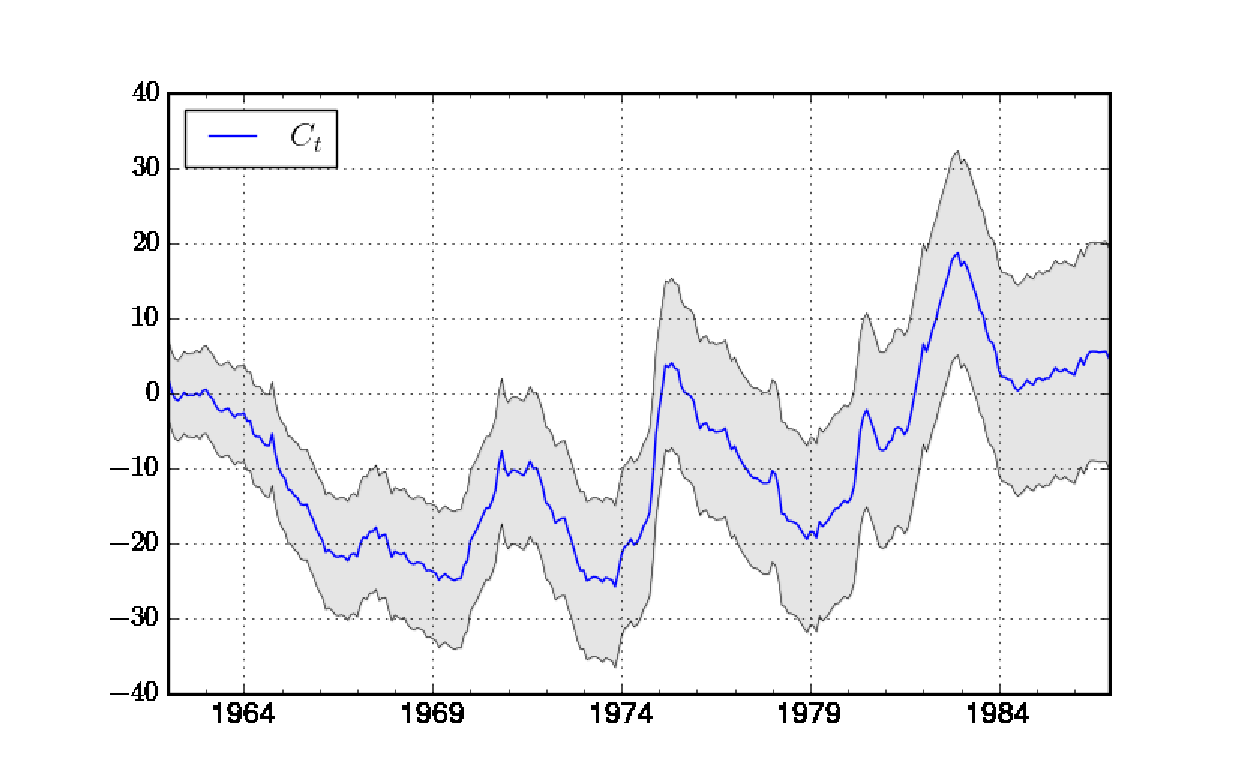
\includegraphics[scale=0.5]{fig/sw_CEI}
\end{figure}
% employees on non agricultural payrolls.
	\subsection{Preliminary analysis}
	
	The first step in specifying the model is to test for whether the series are integrated and, if they are, whether they are cointegrated.  As in \citeA{stock1988probability, stock&watson1989indexes}, for each of the the coincident indicators, \citeA{dickey1979distribution} test for a unit root (against the alternative that the series are stationary, perhaps around a linear time trend) was unable to reject (at the 10\% level) the hypothesis that the series are integrated. P-values are reported in Table \ref{tab:df_pvalues}.
	
	\begin{table}[h!]
		\centering\small
		\captionsetup{width=0.6\textwidth, font=small}
		\caption{P-values of the test \protect\citeA{dickey1979distribution} for a unit root applied to the four series used in the index estimation. We fail to reject in every case at thte 10\%.}\label{tab:df_pvalues}
		\vspace{0cm}
		\begin{tabular}{l|rrrr}

{} &    IP & GMYXP8 &  MT82 & LPMHU \\ \hline\hline

p value &  0.97 &   0.99 &  0.98 &  0.99 \\ \hline\hline

\end{tabular}

	\end{table}
 
	The subsequent aplication of the \citeA{engle1987co} test of the nul hypothesis that the four series are not cointegrated against the alternative of cointegration failed to reject at the 10\% significance level. Thus these tests provided no evidence against the hypothesis that each series is integrated but they are not cointegrated. I therefore estimated the model using for the first diference of the logarithm of each of the coincident series, standardized to have zero mean and unit variance.

	\begin{table}[h!]
		\centering\small
		\captionsetup{width=0.6\textwidth, font=small}
		\caption{P-values of the \protect\cite{engle1987co} for cointegration to the four series used in the index estimation. We fail to reject in every case at the 10\% level.}
		\begin{tabular}{l|rrrr}

{} &        IP &    GMYXP8 &      MT82 &     LPMHU \\ \hline\hline

IP     &       - &  0.013209 &  0.230167 &  0.000807 \\
GMYXP8 &   0.01397 &       - &  0.020279 &  0.128943 \\
MT82   &  0.248144 &  0.020003 &       - &  0.121991 \\
LPMHU  &  0.051041 &  0.134312 &  0.130508 &       - \\ \hline\hline

\end{tabular}

	\end{table}

\subsection{Maximum Likelihood Estimation}

The parameters of the single-index model have been estimated using IP, DPI, TS and AW over the periods 1959:2-1983:12. As in \citeA{stock&watson1989indexes}, a second order autoregressive  specification  has been adopted for $\Delta C_t$, so that $p=2$. Also, errors $u_t$ are modelled as an $AR(2)$, i.e., $k=2$. I have followed \citeA{stock1988probability} and considered $\gamma$ to be constant, i.e., $\gamma = \gamma_0\in\R^4$. The loglikelihood for this model is 424.529. The maximum likelihood estimates of the parameters of the single-index model are presented in Tables  he maximum likelihood estimates of the parameters of the single-index model are presented in Table \ref{tab:sw-ml-params}. I have follow \citeA{gupta1974computational} for maximising the log likelihood.The basic idea is that the negative log likelihood is minimised by the Newton-Raphson Method, iterating the process until the log likelihood stabilises. Standard errors are computed as the square root of the diagonal of the (approximated) Hessian matrix of $\mathcal{L}$.

\begin{table}[h!]
\centering\captionsetup{width=0.8\textwidth, font=small}
\caption{The estimation period is 1959:2-1983:12. The parameters were estimated by Gaussian maximum likelihod as described in the text. The parameters are $\gamma = (\gamma_1,\ldots, \gamma_4)$, $D(L)=\text{diag}\left(d_1(L),\ldots, d_4(L)\right)$, where $d_i(L) = 1-d_{i1}L - d_{12}L^2$ and $\Sigma = \text{diag} \left(1,\sigma_1^2,\ldots,\sigma_4^2\right)$. Maximum likelihood is $\mathcal{L}=424.529$.}\label{tab:sw_ml-params}
\begin{tabular}{l|cccc}
&IP&GMYX&LPMH&LPMHU\\\hline\hline
$\gamma_i$&-0.7219&-0.4976&-0.4625&-0.5001\\
&(0.033)&(0.0283)&(0.0283)&(0.0274)\\
$d_{1i}$&-0.0204&-0.1163&-0.4273&-0.4453\\
&(0.0858)&(0.1191)&(0.0769)&(0.0489)\\
$d_{2i}$&-0.1492&0.1513&-0.2311&-0.1206\\
&(0.1071)&(0.0515)&(0.0996)&(0.0675)\\
$\sigma_i$&0.4681&0.78&0.7425&0.7132\\&(0.0362)&(0.033)&(0.0309)&(0.0308)\\\hline\hline
\end{tabular}
\end{table}
The CEI, $C_{t|t}$,  is is plotted in Figure \ref{fig:cei}. Notice that  $$C_{t|t} = [Z_c \ 0 \ 1] \hat{\alpha}_{t|t}.$$ I have also included a 5\% confidence interval band measured by $$C_{t|t}\pm 1.96 \sqrt{\hat{P}_{t|t}},$$ where $$\hat{P}_{t|t} = [Z_c \ 0 \ 1] \hat{\alpha}_{t|t}[Z_c \ 0 \ 1]^{\text{\tiny T}}$$


%	\begin{table}[h!]
%		\centering\small
%			\captionsetup{width=0.6\textwidth, font=small}
%			\caption{The estimation period is 2006:12-2022:08. The parameters were estimated by Gaussian maximum likelihod as described in the text. The parameters are $\gamma = (\gamma_1,\ldots, \gamma_4)$, $D(L)=\text{diag}\left(d_1(L),\ldots, d_4(L)\right)$, where $d_i(L) = 1-d_{i1}L - d_{12}L^2$ and $\Sigma = \text{diag}\left(1,\sigma_1^2,\ldots,\sigma_4^2\right)$. Maximum likelihood is $\mathcal{L}=274.819$ at the 42688th iteration.}\label{tab:ml-params1}
%		\begin{tabular}{l|rrrr}
%			& IP & DPI & TS & AW \\\hline\hline
%			$\gamma_i$ & 0.592400 & -0.160700 & 0.585400 & 0.320700 \\
%			$d_{1i}$ & -0.136700 & -0.277700 & 0.298100 & -0.857200 \\
%			$d_{2i}$ & -0.010300 & -0.796800 & -0.288700 & -0.060500 \\
%			$\sigma_{i}$ & 0.399400 & 0.611400 & 0.013000 & 0.831200 \\\hline\hline
%			&\multicolumn{2}{c}{$\phi_1$} & \multicolumn{2}{c}{$\phi_1$}  \\\hline\hline
%			&\multicolumn{2}{c}{0.994600} & \multicolumn{2}{c}{0.639000} \\\hline
%		\end{tabular}
%	\end{table}

%	
%
%	\begin{figure}[h!]
%		\centering
%		\captionsetup{width=0.6\textwidth, font=small}
%		\caption{Evolution of the maximum likelihood, $\mathcal{L}$, during the iteration process. X-axis is plotted in log-scale.}
%		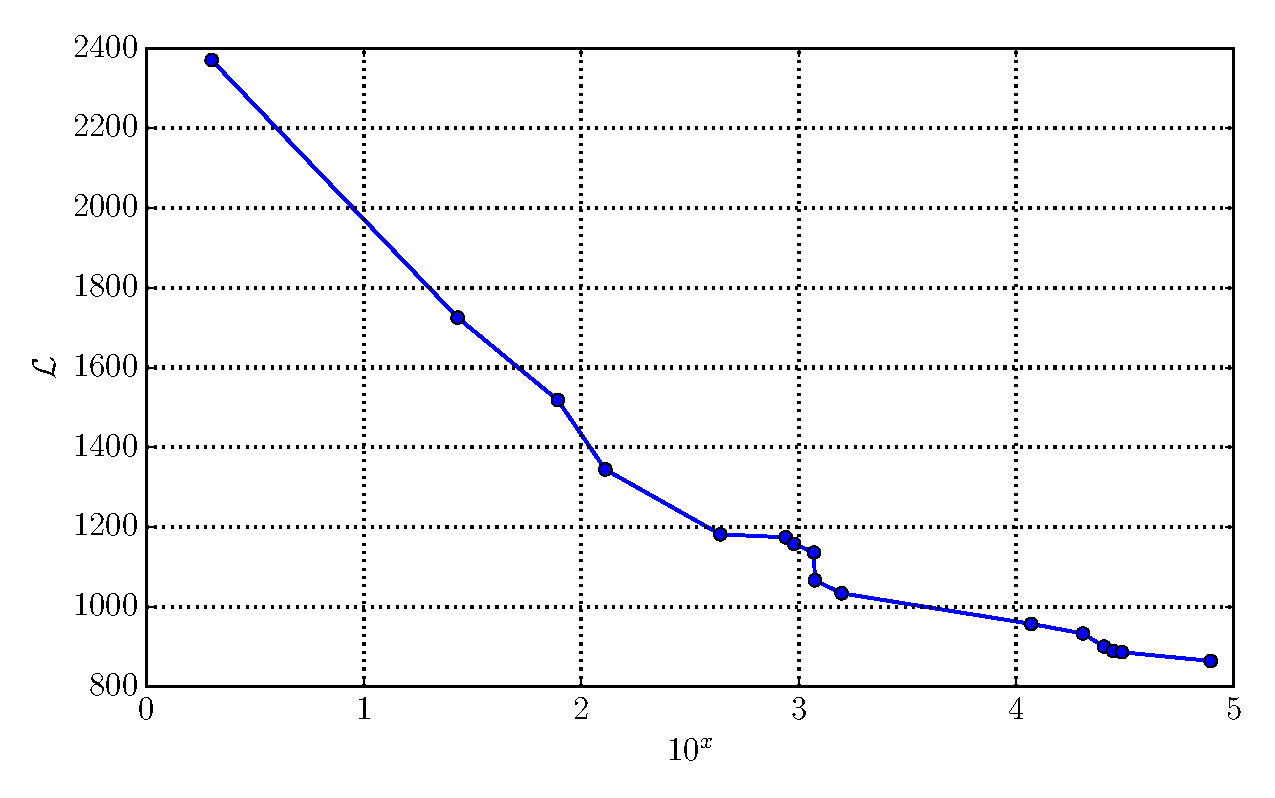
\includegraphics[scale=0.5]{fig/L.eps}
%	\end{figure}
%
%		\begin{figure}[h!]
%		\centering
%		\setlength{\abovecaptionskip}{1pt}
%		\captionsetup{width=0.6\textwidth, font=small}
%		\caption{$C_{t|t} = \begin{bmatrix}
%				Z_c & 0 & 1
%			\end{bmatrix} \alpha_{t|t}$.}
%		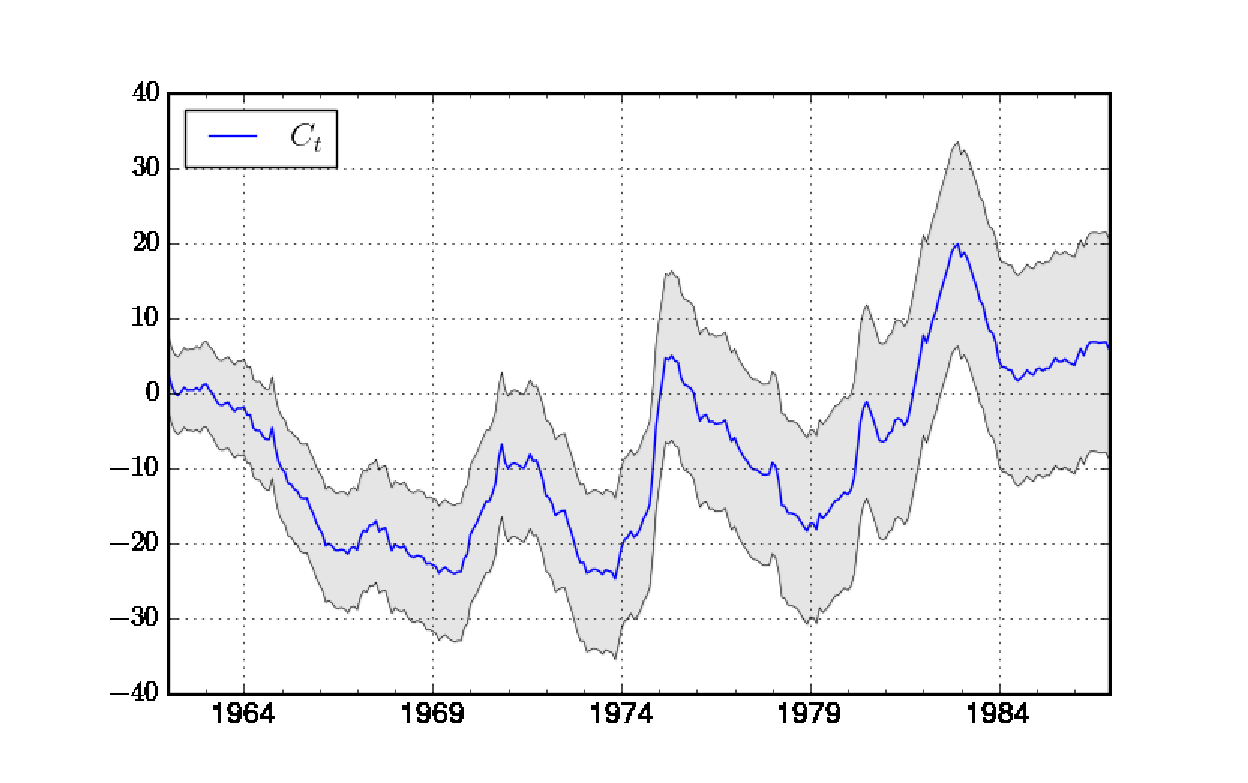
\includegraphics[scale=0.6]{fig/CEI.eps}
%	\end{figure}
% IP: aUSIPMANG/CA
% DPI: aUSGPYDPC/CA
% TS: aUSWSLS/A
% AW: USWRKW=ECI


	\section{The Coincident Index: Empirical Results from 2007:01-2022:12}
		
I want to find the Coincident Economic Index with more recent data. Then, I take US data from Refinitiv on Industrial Production (USIPMANG), total disposable personal incomes (USGPYD), total machinery manufacturing (USPPM), and weekley average work hous in nonfarm payrolls (USWRKW).  I am taking data from 2007:01-2012:12.


\begin{figure}[h!]
	\centering
	\captionsetup{width=0.5\textwidth, font=small}
	\caption{$C_{t|t}$ together with a 5\% confidence interval (assuming gaussianity) using data from 2007:01 to 2022:12.}\label{fig:new_cei}
	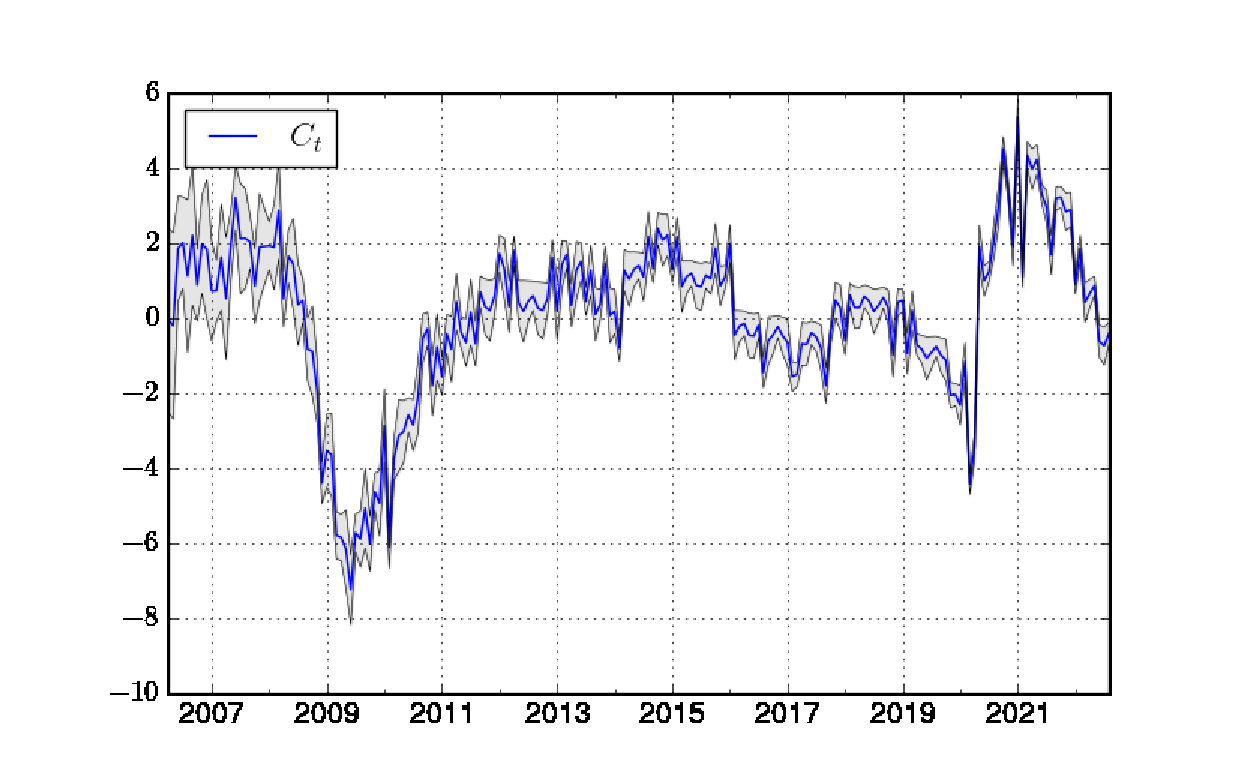
\includegraphics[scale=0.5]{fig/newdata_CEI}
\end{figure}

% employees on non agricultural payrolls.
\subsection{Preliminary analysis}

I repeat the same analysis: I check whether the series are integrated and, if they are, whether they are cointegrated.  For each of the the coincident indicators, \citeA{dickey1979distribution} test for a unit root (against the alternative that the series are stationary, perhaps around a linear time trend) was unable to reject (at the 10\% level) the hypothesis that the series are integrated. P-values are reported in Table \ref{tab:new_df_pvalues}.

\begin{table}[h!]
	\centering\small
	\captionsetup{width=0.6\textwidth, font=small}
	\caption{P-values of the test \protect\citeA{dickey1979distribution} for a unit root applied to the four series used in the index estimation. We fail to reject in every case at thte 10\%.}\label{tab:new_df_pvalues}
	\vspace{0cm}
	\begin{tabular}{l|rrrr}

{} & USIPMANG & USGPYD & USPPM & USWRKW \\ \hline\hline

p value &     0.08 &   0.91 &  0.98 &   0.47 \\ \hline\hline

\end{tabular}

\end{table}

The subsequent aplication of the \citeA{engle1987co} test of the null hypothesis that the four series are not cointegrated against the alternative of cointegration failed to reject at the 10\% significance level. Thus these tests provided no evidence against the hypothesis that each series is integrated but they are not cointegrated. I therefore estimated the model using for the first diference of the logarithm of each of the coincident series, standardized to have zero mean and unit variance.

\begin{table}[h!]
	\centering\small
	\captionsetup{width=0.6\textwidth, font=small}
	\caption{P-values of the \protect\cite{engle1987co} for cointegration to the four series used in the index estimation. We fail to reject in every case at the 10\% level.}
	\begin{tabular}{l|rrrr}

{} &  USIPMANG &    USGPYD &     USPPM &    USWRKW \\ \hline\hline

USIPMANG &       - &  0.131099 &  0.195242 &  0.038813 \\
USGPYD   &  0.961745 &       - &  0.792259 &  0.764748 \\
USPPM    &  0.992393 &  0.118382 &       - &  0.940171 \\
USWRKW   &  0.696816 &  0.452826 &   0.08429 &       - \\ \hline\hline

\end{tabular}

\end{table}

\subsection{Maximum Likelihood Estimation}

The parameters of the single-index model have been estimated using USIPMANG, USGPYD, USPPM, USWRKW over the periods 2007:01-2022:12. I repeat the second order autoregressive  specification  has been adopted for $\Delta C_t$, so that $p=2$. Also, errors $u_t$ are modelled as an $AR(2)$, i.e., $k=2$; and $\gamma$ is assumed to be constant, i.e., $\gamma = \gamma_0\in\R^4$. The loglikelihood for this model is 233.490. The maximum likelihood estimates of the parameters of the single-index model are presented in Table \ref{tab:newdata-ml-params}. The procedure is the same than before.

\begin{table}[h!]
\centering\captionsetup{width=0.8\textwidth, font=small}
\caption{The estimation period is 1959:2-1983:12. The parameters were estimated by Gaussian maximum likelihod as described in the text. The parameters are $\gamma = (\gamma_1,\ldots, \gamma_4)$, $D(L)=\text{diag}\left(d_1(L),\ldots, d_4(L)\right)$, where $d_i(L) = 1-d_{i1}L - d_{12}L^2$ and $\Sigma = \text{diag} \left(1,\sigma_1^2,\ldots,\sigma_4^2\right)$. Maximum likelihood is $\mathcal{L}=233.491$.}\label{tab:newdata-ml-params}
\begin{tabular}{l|cccc}
&USIPMANG&USGPYD&USPPM&USWRKW\\\hline\hline
$\gamma_i$&0.2289&0.133&-0.0059&0.8573\\
&(0.0499)&(0.0611)&(0.0382)&(0.0503)\\
$d_{1i}$&0.2115&-0.5554&0.4363&-0.2912\\
&(0.0613)&(0.0794)&(0.057)&(0.0055)\\
$d_{2i}$&-0.219&-0.1022&0.3789&-0.9998\\
&(0.069)&(0.0699)&(0.0408)&(0.011)\\
$\sigma_i$&-0.9257&-0.8277&0.6663&-0.0\\&(0.0436)&(0.0546)&(0.0342)&(0.0134)\\\hline\hline
\end{tabular}
\end{table}


	

%	ndustrial production
%	(IP),totalpersonalincomelestransferpaymentsin1982dolars(CMYXP8), totalmanufacturingandtradesalesin1982dolars(MT82),andemployeson nonagriculturalpayrols(LPNAG)

%
%	\newpage
%	\section{A probability model of the coincident economic indicators}
%	
%	\subsection*{Abstract}

The Index of Coincident Economic Indicators, currently compiled by the US Department of Commerce, is designed to measure the state of overall economic activity. The index is constructed as a weighted average of four key macroeconomic time series, where the weights are obtained using rules that date to the early days of business cycle analysis. This paper presents an explicit time series model (formally, a dynamic factor analysis or ``single-index'' model) that implicitly defines a variable that can be thought of as the overall state of the economy. Upon estimating this model using data from 1959-1987, the estimate of this unobserved variable is found to be highly correlated with the official Commerce Department series, particularly over business cycle horizons. Thus this model provides a formal rationalisation for the traditional methodology used to develop the Coincident Index. Initial exploratory exercises indicate that traditional leading variables can prove useful in forecasting the short-run growth in this series.

\subsection{Introduction}

Since their initial development in 1938 by Wesley Mitchell, Arthur Burns, and their colleagues at the National Bureau of Economic Research, the Composite Indexes of Coincident and Leading Economic Indicators have played an important role in summarising the state of macroeconomic activity. This paper reconsiders the problem of constructing an index of coincident indicators. We will use the techniques of modern time series analysis to cevelop an explicit probability model of the four coincident variables that comprise the Index of Coincident Economic Indicators (CEI) currently compiled by the Deparment of Commerce (DOC). This probability model provides a framework for computing an alternative coincident index. As it turns out, this alternative index is quantitatively similar  to the DOX index. Thus this probability model provides a formal statistical rationalisation for, and interpretation of, the construction of the DOC CEI. This alternative interpretation complements that provided by the methodology developed by Mitchel and Burns (1938) and aplied by, for example ,Zarnowitz and Boachan (1975).

The model adopted in this paper is based on the  notion that the comovements in many macroeconomic variables have a common element that can be captured by a single underlying, unobserved variable. Tin the abstract, this variable represents the general ``state of the economy''. The problem is to estimate the current state of the economy, i.e., this common element in the fluctuations of key aggregate time series variables. This unobserved variable — the ``state of the economy'' — must be defined before any attempt can be made to estimate it. In technical terms, this requires formualting a probability model that provides a mathematical definition of the unobserved state of the economy. In nontechnical terms, this problem can be phrased as a question: What do the leading indicators lead?

Our proposed answer to this question is given in Section 2. This section presents a parametric ``single-index'' model in whic the state of the economy — referred to as $C_t$ — is an unobserved variable common to multiple aggregate time series. Because this model is linear in the unobserved variables, the Kalman Filter can be used to construct the Gaussian likelihood function and thereby to esitmate the unknown parameters of the model by maximum likelihood. As a side benefit, the Kalman Filter automatically computes the minimum mean square error esitmate of $C_t$ using data through period $t$. This estimate, $C_{t|t}$, is teh alternaitve index of coincident indicators computed using the single-index model.

The singleindex model is estimated using data on industrial production, real personal income, real manufacturing and trade sales, and employment in nonagricultural establishments from 1959 to 1987. The results are reported in Section 3. Also in this section, the estimated alternative index $C_{t|t}$ is compared with the DOC series. The similarity between the two is triking, particularly over business-cycle horizons.

Section 4 presents an initial inevstigation into forecasting the growth of $C_{t|t}$ using a variety of leading or predictive macroeconomic variables. The main conclusion is that a parsimoniously parametrised time series model with $C_{t|t}$ and six leading variables can forecast approximately two-thirds of the variance of the growth in $C_{t|t}$ iver the next six months.

A conceptually distinct forecasting problem is explored in section 5. A traditional focus of business cycle analysis has of course been identifying expansion and contractions. Several recent forecasting exercises have focused on forecasting turning points; see, for example, Hymans (1973), Wecker (1979), Zarnowitz and Moore (1982), Kling (1987), and Zellner, Hong and Gulati (1987). Rather than focusing on turning points, the approach taken in Section 5 is to forecast directly the binary variable representing whether the economy is in recession or expansion six months hence. The main conclusion is that, among the binary-response models considered, expansions can be forecasted fairly reliably, recessions less so. Section 6 concludes.

\subsection{The Coincident Indicator Model: specification and Estimation}

One approach to studying aggregate fluctuations is to pick an important economic time series — say employment or GNP — as the object of interest for subsequent analysis and forecasting. This decided, life becomes relatively easy, since economists have decades of experience constructing models to analyse and to forecast observable time sereies variables. From the perspective of business cycle analysis, however, this approach is rather limited. Individual series measure more or less well-defined concepts, such as teh value of all goods and services produced in a quarter or the total number of individuals working for pay. But these series measure only various facets of the overall state of econoic activity; non measure the sate of the economy (in Burns and mitchell's (1946) terminoly, the ``reference cycle'') directly. Moreover, even the concepts that the series purport to measure are measured with error\footnote{Most modern research on the forecasitng potential of the index of leading indicators has focused on its ability to forecast not the reference cycle, but some observable series such as industrial production or unemployment (e.g., Stekler and Schepsman (1973), Vaccara and Zarnowitz (1978), Sargent (1979), Auerbach (1982), and Koch and Rassche (1988)). Our perspective is closer to that underlying the work of Diebold and Rudebusch (1987) and Hamilton (1987). For a historical review of the development of the leading indicators, see Moore (1979).}.

The formulation developed here is based instead on the assumption that there is a single unobserved variable common to many macroeconomic time series. This places Burns and Mitchell's (1946) reference cycle in a fully specified probability model. The proposed model is a parametric version of the ``single-index'' models discussed by Sargent and Sims (1977), in which the single unobserved index is common to multiple macroeconomic variables. Estimated of this unobserved index, constructed using variables that move contemporaneously with this index, provide an alternative index of coincident indicators. This index can then be forecasted using leading variables.

\subsubsection{The Single-Index Model}

Let $X_t$ denote a $n\times 1$ vector of macroeconomic time series variables that are hypothesised to move contemporaneouslly with overall economic conditions. In the single-index model, $X_t$ consists of two stochastic components: the common unobserved scalar time series variable, or `ìndex'', $C_t$, and a $n$-dimensional component that represents idiosyncratic movements in the series and measurement error,~$v_t$. Both the unobserved index and the idiosyncratic component ar modeled as having linear stochastic structures. In addition, $C_t$ is assumed to enter each of the variables contemporaneously. This suggests the formulation:

\begin{align}
		X_t &= \beta\ones + \gamma C_t \ones + v_t \label{eq:model_eq1}\\
		\tilde{\phi}(L) C_t &= \delta + \eta_t \\
		\tilde{D}(L) v_t &= \varepsilon_t\label{eq:model_eq3}
	\end{align}
where $L$ denotes the lag operator, $\phi(L)$ is a scalar lag polynomials, and $D(L)$ is a lag polynomial matrix. According to (\ref{eq:model_eq1}), $C_t$ enters each of the $n$ equations in (\ref{eq:model_eq1}), although varying lags and weights.

As an empirical matter, many macroeconomic time series are well characterised as contianing stochastic trends; see, for example, Nelson and Plosser (1982). A theoretical possibility is that these stochastic trends would enter through $C_t$; in this case, each element of $X_t$ would contain a stochastic trend, but this trend would be common to each element. Thus $X_t$ would be cointegrated of order $k-1$ as defined by Engle and Granger (1987). Looking ahead to the empirical results however, this turns out not to be the case: while we cannot reject the hypothesis that the coincident series we consider individually contain a stochastic trend, neither can we reject the the hypothesis that there is no cointegration among these variables. The system (\ref{eq:model_eq1})-(\ref{eq:model_eq3}) is therefore reformulated in terms of teh changes (or, more precisely, the growth rates) of the variables. Specifically, assume that $\phi(L)$ and $D(L)$ can befactored so that $\tilde{\phi}(L) = \phi(L)\Delta$ and $\tilde{D}(L) = D(L) \Delta$, where $\Delta = 1-L$. Let $Y_t = \Delta X_t$, and $u_t = \Delta v_t$, so that (\ref{eq:model_eq1})-(\ref{eq:model_eq3}) becomes:
\begin{align}
	Y_t &= \beta \ones + \gamma \Delta C_t \ones + u_t \label{eq:model_eq4}\\
	\phi(L) C_t &= \delta + \eta_t \label{eq:model_eq5}\\
	D(L) u_t &= \varepsilon_t\label{eq:model_eq6}
\end{align}
In practice, $X_t$ will be a vector of the logarithms of time series variables so that $Y_t$ is a vector of their growth rates. The lag polynomials $\phi(L)$ and $D(L)$ are assumed to have finite orders $p$ and $k$, respectively. 

The main identifying assumption in the model expresses the core notion of the single-index model that the comovements of the multiple time series arise from the single source $C_t$. This is made precise by assuming that $\left(u_{1,t},\ldots, u_{n,t}, \Delta C_t\right)$ are mutually uncorrelated at all leads and lags. When there are four or more variables, this imposes testable overidentifying restrictions which will be examined empirically below. This is achieved by assuming that $D(L)$ is diagonal and that the $n+1$ disturbances are mutually uncorrelated:
\begin{equation}
	D(L) = \text{diag}\left(d_1(L), \ldots, d_n(L)\right)
\end{equation}
and
\begin{equation}
	\E\left((\eta_t, \varepsilon_t)'(\eta_t,\varepsilon_t)\right) = \text{diag}\left(\sigma_\eta^2, \sigma^2_{\varepsilon_1},\ldots, \sigma^2_{\varepsilon_n}\right)
\end{equation}
In addition, the scale of $\Delta C_t$ is identifying by setting $\sigma^2(\eta_t)=1$. This is a normalisation with no substantive implications.

A final identifying assumption is required to estimate the mean growth rate for $C_{t|t}$. This mean is calculated here as a weighted average of the growth rates of the constituent series. The weigths are those implicitly used to construct $\Delta C_{t|t}$ from the original data series. That is, in this model, $\Delta C_{t|t}$ can be written 
\begin{equation}
	\delta = W(L) Y_t,
\end{equation}
where $W(L)$ is a $1\times n$ lag polynomial vector. The mean of $\Delta C_{t|t}$ equals $W(1)'\mu_Y$, where $W(1) = \sum_{i\geq 0}W_i$ and $\mu_Y$ denotes the mean of $Y_t$. This implies 
\begin{equation}
	\delta = \phi(1) W(1)'\mu_Y.
\end{equation}
Taken together, these assumptions provide sufficient identifying restrictions to estimate the unknown parameters of the model and to extract estimates of $C_t$.

\subsubsection{State Space Representation}

The first step towards estimating the model (\ref{eq:model_eq4})-(\ref{eq:model_eq6}) is to cast into a state space form so that the Kalman Filter can be used to evaluate the likelihood function. This formulation has two parts, the state equation and the measurement equation. The state equation describes the evolution of the unobserved state vector, which contains $\Delta C_t$, $u_t$ and their lags. The measurement equations relates the observed variables to the elements of the state vector. 

The transition equation obstains by combining (\ref{eq:model_eq5}) and (\ref{eq:model_eq6}). Because the objective is to estimate the elvel of $C_t$ using information up to time $t$, it is convenient to augment these equations at this point by the identity $C_{t-1} = \Delta C_{t-1} + C_{t+2}$. The transition equation for the state is thus given by
\begin{equation}\label{eq:transition_eq}
	\begin{bmatrix}
		C_t^\ast \\ u_t^\ast \\ C_{t-1}
	\end{bmatrix}
	=
	\begin{bmatrix}
		\Phi^\ast & 0 & 0 \\ 0 & D^\ast & 0 \\ Z_c & 0 & 1
	\end{bmatrix}
	\begin{bmatrix}
		C_{t-1}^\ast \\ u_{t-1}^\ast \\ C_{t-1}
	\end{bmatrix}
	+ 
	\begin{bmatrix}
		Z_c & 0 \\ 0 & Z_u \\ 0 & 0
	\end{bmatrix}
	\begin{bmatrix}
		\eta_t \\ \varepsilon_t
	\end{bmatrix}
\end{equation}
where 
\begin{equation}
	\begin{aligned}
		C_{t}^\ast &= 
		\begin{bmatrix}
			\Delta C_t &	\Delta C_{t-1} &\cdots \Delta C_{t-p+1}
		\end{bmatrix}'
	\\
		u_t^\ast &= 
		\begin{bmatrix}
		u_t' & u_{t-1}' & \cdots & u_{t-k+1}'
		\end{bmatrix}'
	\\
		\Phi^\ast &=
		\begin{bmatrix}
			\begin{matrix}
			\phi_1 & \cdots  &\phi_{p-1} &
			\end{matrix} & \phi_p\\
			I_{p-1} & 0 
		\end{bmatrix}
	\\
		D^\ast &=
		\begin{bmatrix}
			\begin{matrix}
				D_1  & \cdots & D_{k-1} 
			\end{matrix}& D_k\\
		I_{n(k-1)} & 0 
		\end{bmatrix}
\end{aligned}
\end{equation}
and
\begin{equation}
	\begin{aligned}
		Z_c & = \begin{bmatrix}
			1 & 0_{1\times(p-1)}
		\end{bmatrix}\\
		Z_u & = \begin{bmatrix}
			I_n & 0_{n\times n (k-1)}
		\end{bmatrix}
	\end{aligned}
\end{equation}
and where $I_n$ denotes the $n\times n$ identity matrix, $0_{n\times k}$ denotes a $n\times k$ matrix of zeros, and $D_i = \text{diag}(d_{1,i}, \ldots, d_{n,i}$), where $d_j(L) = 1- \sum_{i=1}^k d_{j,i} L^i$.

The measurement equation is obtained by writing (\ref{eq:model_eq4}) as a linear combination of the state vector:
\begin{equation}\label{eq:measurement_eq}
	Y_t = \beta \ones + \begin{bmatrix}
		\gamma Z_c \ones & Z_u & 0 
	\end{bmatrix}
	\begin{bmatrix}
		C_t^\ast\\u_t^\ast \\ C_{t-1}
	\end{bmatrix}
\end{equation}
The system (\ref{eq:measurement_eq}) and (\ref{eq:transition_eq}) can be rewritten more compactly in the standard form
\begin{align}
	\alpha_t & = T_t \alpha_{t-1} + R\zeta_t \label{eq:alpha}\\
	Y_t & = \beta \ones + Z\alpha_t + \xi_t\label{eq:Y}
\end{align}
where
\begin{equation}
	\begin{aligned}
		\alpha_t &= \begin{bmatrix}
			(C_t^\ast)' & (u_t^\ast)' & C_{t-1}'\\
		\end{bmatrix}'\\
		\zeta_t & = \begin{bmatrix}
		\eta_t & \varepsilon_t'
	\end{bmatrix}'
	\end{aligned}
\end{equation}
and where $T_t$, $R$ and $Z$ respectvely denote the transition matrix in (\ref{eq:transition_eq}), the selection matrix in (\ref{eq:transition_eq}), and the selection matrix in (\ref{eq:measurement_eq}). The covariance matrix of $\zeta_t$ is $\E\zeta_t\zeta_t'=\Sigma$. For generality, a measurement error term $\xi_t$ (assumed uncorrelated with $\eta_t$) has been added to the measurement equation (\ref{eq:Y}), and the transition matrix $T_t$ is allowed to vary over time. In empirical work below, however, the measurment noise is set to zero and the time invariant transition matrix in (\ref{eq:transition_eq}) is used\footnote{The state space representation (\ref{eq:measurement_eq}) and (\ref{eq:transition_eq}) is not unique. In practice, it is computationally more efficient to work with a lower dimensional state vector. This can be achieved by filtering $Y_t$, $\gamma\Delta C_t$ and $u_t$ in (\ref{eq:model_eq4}) by $D(L)$ and treating $\varepsilon_t$ as a measurement error. The resulting state vector has dimension $p+1$}.

\subsubsection{Estimation}

The Kalman Filter is a well-known way to compute the Gaussian likelihoodo function for a trial set of parameters; for a discusion, see Harvey (1981). The filter recursively constructs minimum mean square error (MSE) estimates of the unobserved state vector, given observations on $y_t$. The filter consists of two set of equations, the prediction and updating equations. Let $\alpha{t|\tau}$ denote the estimate of $\alpha_t$ based on $(y_1,\ldots, y_\tau)$, let $\E[\xi_t\xi_t'] = H$, and recall that $\E[\zeta_t\zeta_t'] = \Sigma$. Also, let $P_{t|\tau} = \E\left[\left(\alpha_{t|\tau}-\alpha_t\right)\left(\alpha_{t|\tau}-\alpha_t\right)'\right]$. With this notation, the prediction equations of the Kalman filter are:
\begin{align}
	\alpha_{t|t-1} &= T_t \alpha_{t-1|t-1}\label{eq:KF_eq12}\\
	P_{t|t-1} &= T_t P_{t-1|t-1}T_t' + R\Sigma R'\label{eq:KF_eq13}
\end{align}
The forecast of $Y_t$ at time $t-1$ is $Y_{t|t-1} = \beta\ones + Z\alpha_{t|t-1}$, and the forecast error is $\nu_t=Y_t-\beta\ones - Z\alpha_{t|t-1}$. The updating equations of the filter are:
\begin{align}
	\alpha_{t|t} &= \alpha_{t|t-1} + P_{t|t-1} Z'F_t^{-1}\nu_t\label{eq:KF_eq14}\\
	P_{t|t}& = P_{t|t-1} - P_{t|t-1}Z'F_t^{-1} Z P_{t|t-1}\label{eq:KF_eq15}
\end{align}
where $F_t = \E[\nu_t\nu_t'] = Z P_{t|t-1}Z' + H$. 

The Kalman Filter equations (\ref{eq:KF_eq12})-(\ref{eq:KF_eq15}) permit recursive calculation of the predicted state vector, $\alpha_{t|t-1}$, and of the covariance matrix of this estimate, $P_{t|t-1}$, given the assumed parameters in $T_t$, $R$, $\Sigma$, $H$, and $Z$, and given initial values for $\alpha_{t|t}$ and $P_{t|t}$. For exact maximum likelihood estimation, these initial values are taken to be the unconditional expectation of $\alpha_t$ and its covariance matrix, $\E[(\alpha_t-\E\alpha_t)(\alpha_t-\E\alpha_t)']$; that is, $\alpha_{0|0}=0$, and $P_{0|0} = \sum_{j\geq 0} T_{t-j}^j \Sigma T_{t-j}^j$. Alternatively, one could set $P_{0|0}$ to an arbitrary constant matrix. In this case, the estimates are asymptotically equivalent to maximum likelihood.

The Gaussian log likelihood is then computed (up to an additive constant) as:
\begin{equation}
	\mathcal{L} = \frac{1}{2}\sum_{t=1}^T \nu_t' F_{t}^{-1}\nu_t - \frac{1}{2}\sum_{t=1}^T \log \det F_t.
\end{equation}
The Gaussian maximum likelihood estimates of the parameters are found by maximising $\mathcal{L}$ over the parameter space.
	
% \section{Appendix}
%	
Let $X_t\in\R^n$ be  a vector of logarithms of macroeconomics variables which are  hypothesed to move together with overall economic conditions. Also, $X_t$ consists of two stochastic components:
\begin{enumerate}
	\item The common unobserved scalar variable, $C_t$, which is the `ìndex''.
	\item An idiosyncratic component, $u_t\in\R^n$ which is assumed to represent also the potential measurement error.
\end{enumerate}
Both components are assumed to having linear stochastic structures. The coincident variables used in the analysis are integrated but not cointegrated. Hence, the model is specified in terms of $\Delta X_t$ and $\Delta C_t$. Now we can write the model:
\begin{equation}\label{eq:model1}
	\begin{aligned}
		\Delta X_t &= \beta + \gamma(L) \Delta C_t + u_t \\
		D(L) u_t &= \varepsilon_t \\
		\phi(L) \Delta C_t &= \delta + \eta_t
	\end{aligned}
\end{equation}
Here $L$ denotes the lag operator, and $\phi(L)$, $\gamma(L)$, and $D(L)$ are, respectively, scalar, vector, and matrix lag polynomials.

\assumption The co-movements of the multiple time series arise from the source $\Delta C_t$.

This assumptions holds by assuming that $\left(u_t^1,\ldots, u_t^n, \Delta C_t\right)$ are (mutually) uncorrelated at all leads and lagas, which is achieved by making $D(L)$ diagonal and the $n+1$ disturbances $\left(\varepsilon_t^1,\ldots, \varepsilon_t^n, \Delta C_t\right)$ mutually and serially uncorrelated.

\assumption $\gamma(L) = \gamma_0$. This is done in order to restrict the impulse response from $\eta_t$ to $\Delta X_t$ to be proportional across the observable variables. This is done in the case where there are \emph{more than three} observable series or when the variables are serially correlated. See page 344 in \citeA{stock&watson1989indexes}.

Let's assume also, without loss of generality, that $\phi_0 = D_0 = 1$. Hence, we can rewrite (\ref{eq:model1}) as

\begin{equation}\label{eq:model2}
	\begin{aligned}
		\Delta X_t &= \beta + \gamma \Delta C_t + u_t \\
		\Delta C_t &= \delta + \sum_{i=1}^p D_i \Delta C_{t-i} + \eta_t\\
		u_t & = \sum_{i=1}^q \phi_i u_{t-i} + \varepsilon_t
	\end{aligned}
\end{equation} 
Let me now consider the notation $v^{1,k}$ for a vector whose numbers are already known and therefore it represents $(v_1,\ldots, v_k)$. Hence, we can rewrite (\ref{eq:model2}) as
\begin{equation}\label{eq:model3}
	\begin{aligned}
		\Delta X_t &= \beta + \gamma \Delta C_t + u_t \\
		\Delta C_t &= \delta + \phi^{1,p}\cdot  \Delta C_{t}^{1,p}+ \eta_t\\
		u_t & = D^{1,q}\cdot u_t^{1,q}+ \varepsilon_t,
	\end{aligned}
\end{equation}
chere the dot stands for the scalar product. Hence, we can write the second and third equations in (\ref{eq:model3}) as a matrix equation for the \emph{transition equation} of the Kalman filter that we want to construct.
\begin{equation}
	\begin{bmatrix}
		C_{t}^\ast  \\ u^\ast_t
	\end{bmatrix}
	=
	\begin{bmatrix}
		\delta \\ 0
	\end{bmatrix}
	+
	\begin{bmatrix}
		\phi^\ast & 0 \\
		0 &D^\ast  
	\end{bmatrix}
	\begin{bmatrix}
		C_{t-1}^\ast \\ u_{t-1}^\ast\\
	\end{bmatrix}
	+
	\begin{bmatrix}
		Z_c' & 0 \\ 0 & Z_u'
	\end{bmatrix}
	\begin{bmatrix}
		\eta_t \\ \varepsilon_t
	\end{bmatrix}
\end{equation}
where $Z_c = e_1\in\R^p$ (i.e., one in the first entry and zeros in the rest $p-1$); $Z_u = e_1\in\R^q$ (i.e., one in the first entry and zeros in the rest). Regarding the first equation, which is suppose to be the measurement equation, we can write it as
\begin{equation}
	\Delta X_t 
	=
	\beta + 
	\begin{bmatrix}
		\gamma Z_c & Z_u 
	\end{bmatrix}
	\begin{bmatrix}
		C_{t}^\ast \\ u_{t}^\ast
	\end{bmatrix}
\end{equation}

To sum up, we can write everything as 
\begin{equation}
	\begin{aligned}
		y_t &= d + Z\alpha_t \\
		\alpha &= c + T\alpha_{t-1} + R\eta_t,
	\end{aligned}
\end{equation}
with $d=\beta$, $c=(\delta, 0)$, and
\begin{equation}
	Z = \begin{bmatrix}
		\gamma Z_c & Z_u 
	\end{bmatrix}, \quad\quad T = \begin{bmatrix}
		\phi^\ast & 0 \\
		0 &D^\ast  
	\end{bmatrix}, \quad\quad R = \begin{bmatrix}
		Z_c' & 0 \\ 0 & Z_u'
	\end{bmatrix}
\end{equation}

The system is estimated by maximum likelihood using the Kalman filter. The proposed CEI si computed as the minimum mean square error linear estimate of this single common factor, $C_{t|t}$, produced by applying the Kalman filter to the estimated system, i.e., it is a linear combination of current and past logarithms of the coincidents variables.

\subsection{Data}

The proposed CEI is based on four series:
\begin{enumerate}
	\item Industrial Production. I am using the index.
	\item Real Personal Income less transfer payments.
	\item Real manufacturing and trade sales.
	\item Employee-hours in nonagricultural establishments.
\end{enumerate}
	\newpage
	\bibliographystyle{apacite}
	\bibliography{main}
\end{document}